


\chapter{NBODY6}
\label{App:nbody6}

NBODY6 is the second youngest iteration of the NBODY family, a suite of n-body integrators created by Sverre Aarseth. It can compute the gravitational interaction between up to 128,000 stars in a collisional fashion, meaning there is no softening of the potential, at any scale. This allows for very close binaries to form and remain in the system. To achieve its impressive performances, NBODY6 relies on several optimization technique which have been first developed in the 1960s and 1970s, and improved ever since. Here will be developped four major features of NBODY6, in chronological order of their implementation: block time-step, KS-regularization, Hermite scheme and Ahmad-Cohen neighbour scheme. A full description can be found in Sverre Aarseth's book \citep{Aarseth2003}. Inspiration for this section should be credited to the user manual of NBODY6++, written by Emil Khalisi and Rainer Spurzem.

%\section{H\'enon units}
%
%NBODY6 uses a set of units specifically invented for the Nbody gravitational problem, the Nbody units, or H\'enon units (as prescribed by Douglas Heggie during the MODEST 2014 meeting). These units are based on three relations:
%
%\begin{align}
%G &= 1\\
%M_t &= 1\\
%E &= -\frac{1}{4}
%\end{align}
%
%With $G$ the gravitational constant, $M_t$ the total mass of the system and $E$ total energy of the system. For a virialized system, that is a relaxed system in which the virial ratio 
%\begin{equation}
%Q = - \frac{E_k}{E_p} = 0.5
%\end{equation}
%it comes that $E_k=0.25$ and $E_p = -0.5$ and, considering the definition of the virial radius 
%\begin{equation}
%R_v = - \frac{G M_t^2}{2 E_p} = 1.
%\end{equation} 
%
%This unit system was designed for virialized systems, but can be used for out of equilibrium systems, as long as they are bound ($Q <1$), with energy expressions functions of $Q$
%\begin{align}
%E_p  &= - \frac{1}{4(1-Q)}\\
%E_k &= \frac{Q}{4(1-Q)}
%\end{align}
%which still fulfills the $E = -\frac{1}{4}$ condition. In practice, the H\'enon mass, radius and velocities are obtained through
%
%\begin{align}
%m_h &= \frac{m}{M_t}\\
%r_h &= 4 (1-Q) |E_p| \cdot r\\
%v_h &= \sqrt{ \frac{Q}{4(1-Q) E_k} } \cdot v
%\end{align}
%
%with $E_p$ and $E_k$ being computed before rescaling with H\'enon masses and $G=1$. Such a system can be used as an input for NBODY6 without the need for the software to rescale anything.
\section{Block time-step}
 
In the first Nbody simulations, the system was integrated with an universal time-step, determined by the most accelerated star. A star in the outer regions of the cluster with a small velocity did not need to be updated that often. One of the first improvement  was the introduction of individual time-step: each star is attributed its own time-step, depending on the force that is applied to it and its derivatives:

\begin{equation}
\label{Eq:0_timestep}
\Delta t_i =  \eta \sqrt{\frac{ |\bold{F_i}||\bold{F^{(2)}_i}| + |\bold{F^{(1)}_i}|^2 }{|\bold{F^{(1)}_i}||\bold{F^{(3)}_i}| + |\bold{F^{(2)}_i}|^2}}
\end{equation}
 
With $\bold{F}^{(j)}_i$ begin the j-th derivative of the force applied to particle i and $\eta$ a user-defined accuracy parameter. Such a complex formulation is the result of extensive tests and is quite robust for many special cases. Individual time-steps leads to desynchronized particles, hence the need to interpolate the positions of other particles to compute $\bold{F}_i$, which was achieved through fourth-order polynoms.
 
 To limit the amount of desynchronization, block-time steps were introduced. Instead of having as many time steps as particles, one only allows quantized power of 2 of an initial time step. $\Delta t_0$,$\frac{\Delta t_0}{2}$, $\frac{\Delta t_0}{4}$, $\frac{\Delta t_0}{2^i}$. All time steps are then commensurate and regularly fall back on the same time steps, minimizing the amount of interpolation during the force calculations. The concept is illustrated on Fig~\ref{Fig:0_blocktimesteps}.
 
\begin{figure}

\center
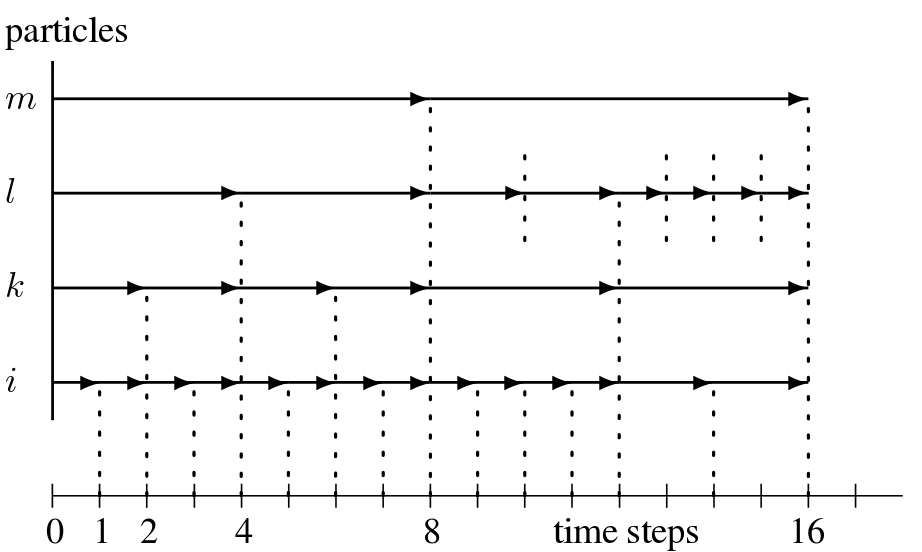
\includegraphics[width=0.6\linewidth]{Figures/0_block_timesteps.png}
\caption[Illustration of block time steps on 4 particles]{Illustration of block time steps on 4 particles. Particles get their positions updated for each arrow symbol, common time steps are shown as vertical dotted lines. Figure from NB6++ User Manual. }
\label{Fig:0_blocktimesteps}
\end{figure} 
 
 
\section{KS-regularization}

Close binaries are extremely problematic in N-body simulations. They require a small time step as both binary components are much more accelerated than any other stars in the system, while the rest of the system is unaffected. Block time-step mitigate this problem, but the binary system still requires a lot of integration for an orbit that is essentially already known. Regularization is an answer to this problem. The essence of regularization is to decouple the integration of a sufficiently isolated sub-system, changing its coordinates to make integration easier, and including perturbations from external bodies. Several regularization scheme exist, NBODY6 implemented the Kustaanheimo-Stiefel method, or KS \citep{KS1965}.

Two bodies are candidates for regularization when their impact parameter is lower that the one needed for an orthogonal deviation, wherein their trajectory are deviated of 90$^\circ$:
\begin{equation}
b_\perp = 2G \frac{m_1 +m_2}{v^2_\infty}
\end{equation}
with $m_i$ components masses and $v_\infty$ relative velocity before encounter. This impact parameter can be converted to a time step computed through equation ~\ref{Eq:0_timestep}:
\begin{equation}
dt_{min} = \kappa \frac{\eta}{0.03} \left( \frac{r^3_{min}}{\langle m \rangle}\right)^\frac{1}{2}.
\end{equation}

To be actually regularized, two bodies have to have a mutual time step lower than $dt_{min}$ and fulfill two conditions:

\begin{align}
\bold{R_r} \cdot \bold{V_r} &> 0.1 \sqrt{ G(m_1+m_2)R_r}\\
\label{Eq:0_KSperturbation}
\frac{\left| \Delta \bold{F_r} \right| \cdot R^2_r}{G(m_1+m_2)} &< 0.25.
\end{align}

$\bold{R_r}$ and $\bold{V_r}$ being the relative velocities and positions of the particles and $\left| \Delta \bold{F_r} \right|$ the differential force applied to them, or perturbation. These conditions mean the subsystem is dynamically decoupled from external influence, but not unperturbed. When they are satisfied, the subsystem is regularized: components are fused in a single particle at the system's center of mass in the global system, while the internal dynamics of the pair and computed separately, with a set of changed coordinates. These coordinates are tailored for binary motion and close approach, they are well behaved when $R_r \rightarrow 0$. The influence of perturbers is taken into account when necessary. When the perturbation ratio (left hand side of equation~\ref{Eq:0_KSperturbation}) drops below a certain value, the system is considered isolated and it is not computed anymore, its parameters being stored until the perturbation is strong enough to warrant integration.

Regularisation have been extended to 3 and 4 bodies in hierarchical subsystems. NBODY6 can handle the regularization of a small-n non-hierarchical subsystem following the chain algorithm, see \cite{Mikkola1993}.


\section{Hermite integration scheme}

On the appropriate time-scales, the accelerations of the particles in a nbody system vary smoothly. It is therefore possible to predict the future acceleration then to correct the prediction, achivieving high order integration with limited computational cost. The Hermite integration scheme was first  introduced by \cite{Makino1991} and has since been implemented within NBODY6 \citep{Aarseth2003,Nitadori2012}.

%Using individual time steps, the standard integration algorithm starts by determining the next particle whose motion to integrate, that is the one whose integration step will bring us to the smaller time: $ i = min_j(t_j + \Delta t_j)$.

The first step is to compute the acceleration and its derivative at $t=t_0$ , for all particles $i$:

\begin{figure}
\center
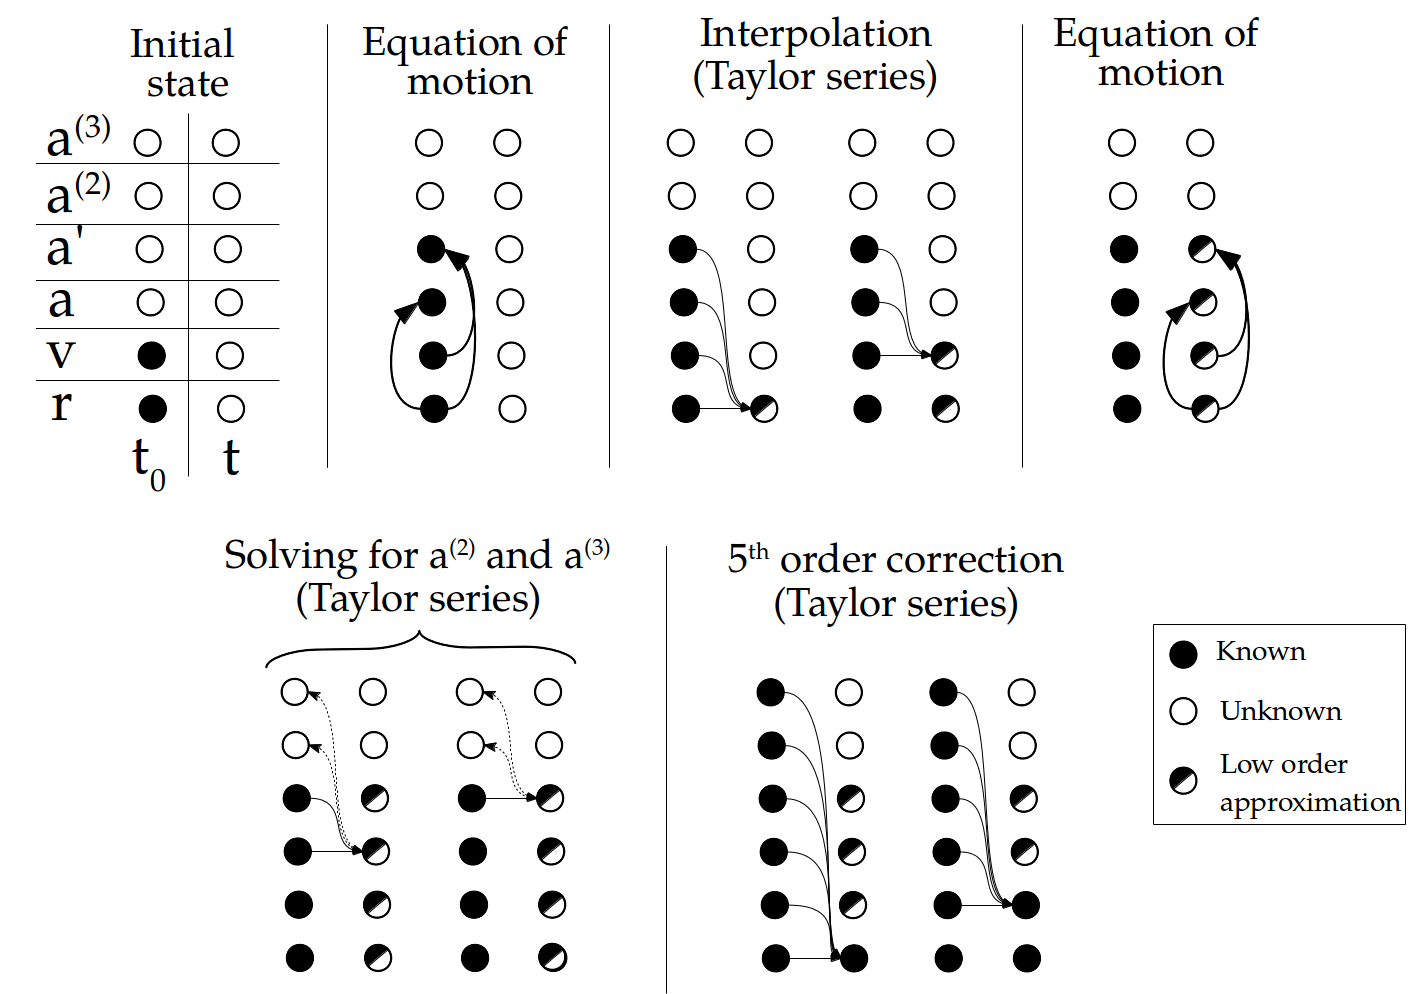
\includegraphics[width=0.9\linewidth]{Figures/0_hermite_scheme.png}
\caption[Summary of the Hermite integration scheme]{Summary of the Hermite scheme starting from known positions and velocities at $t_0$ to obtain 5th order values at t.}
\label{Fig:0_hermite_scheme}
\end{figure} 
 

\begin{align}
\label{Eq:0_Hermite_acc1}
\bold{a}_{0,i} &= - \sum\limits_{i\neq j} G m_j \frac{\bold{R}}{R^3}\\
\label{Eq:0_Hermite_acc2}
\dot{\bold{a}}_{0,i} &=  - \sum\limits_{i\neq j} G m_j \left[ \frac{\bold{V}}{R^3}  + 
	\frac{ 3 \bold{R} ( \bold{V} \cdot \bold{R} )  }{R^3}\right]
\end{align}
with $\bold{R} = \bold{r}_{0,i} - \bold{r}_{0,j} $ and $\bold{V} = \bold{v}_{0,i} - \bold{v}_{0,j} $. Using these quantities, it is now possible to predict the positions and velocities at $t$ through a Taylor serie, again for all particles $i$:

\begin{align}
\bold{r}_{p,i}(t) &= \bold{r}_0 + \bold{v}_0 (t-t_0) + \bold{a}_{0,i}\frac{(t-t_0)^2}{2!} 	
		 +\dot{\bold{a}}_{0,i}\frac{(t-t_0)^3}{3!}\\
\bold{v}_{p,i}(t) &= \bold{v}_0 + \bold{a}_{0,i}(t-t_0) + \dot{\bold{a}}_{0,i}\frac{(t-t_0)^2}{2!}
\end{align}.

The predicted accelerations and their derivatives $\bold{a}_{p,i}(t)$,  $\dot{\bold{a}}_{p,i}(t)$ are computed by injecting $\bold{r}_{p,i}(t)$ and $\bold{v}_{p,i}(t)$ into equations \ref{Eq:0_Hermite_acc1} and \ref{Eq:0_Hermite_acc2}. The accelerations at t, of which predicted values have just been computed, can also be obtained through Taylor series:

\begin{align}
\label{Eq:0_Hermite_taylor1}
\bold{a}_{i}(t) &= \bold{a}_{0,i} + \dot{\bold{a}}_{0,i} (t-t_0) + \bold{a}^{(2)}_{0,i}\frac{(t-t_0)^2}{2!} + \bold{a}^{(3)}_{0,i}\frac{(t-t_0)^3}{3!}\\
\label{Eq:0_Hermite_taylor2}
\dot{\bold{a}}_{i}(t) &=  \dot{\bold{a}}_{0,i} +  \bold{a}^{(2)}_{0,i}(t-t_0) + \bold{a}^{(3)}_{0,i}\frac{(t-t_0)^2}{2!}
\end{align}
with $\bold{a}^{(2)}_{0,i}$,$\bold{a}^{(3)}_{0,i}$ the third and fourth derivative of the acceleration at $t=0$. Note that these quantities are unknown for now. To take the derivatives of equation \ref{Eq:0_Hermite_acc2} would be too computationnaly expansive. Instead, $\bold{a}_{p,i}(t)$ and  $\dot{\bold{a}}_{p,i}(t)$ are injected in the left hand side of equations \ref{Eq:0_Hermite_taylor1} and \ref{Eq:0_Hermite_taylor2} and solved for $\bold{a}^{(2)}_{0,i}$ and $\bold{a}^{(3)}_{0,i}$. This leads to the expressions:

\begin{align}
\bold{a}^{(3)}_{0,i} &= 12 \frac{\bold{a}_{0,i} - \bold{a}_{p,i}}{(t-t_0)^3} +6 \frac{\dot{\bold{a}}_{0,i} - \dot{\bold{a}}_{p,i}}{(t-t_0)^3}\\
\bold{a}^{(2)}_{0,i} &= -6 \frac{\bold{a}_{0,i} - \bold{a}_{p,i}}{(t-t_0)^2} - 2 \frac{2\dot{\bold{a}}_{0,i} + \dot{\bold{a}}_{p,i}}{t-t_0}.
\end{align}

The predicted values of positions and velocities are then corrected using the second and third order derivatives of acceleration, yeilding fifth order accurate values.

\begin{align}
\bold{r}_{c,i}(t) &= \bold{r}_{p,i}(t) + \bold{a}^{(2)}_{0,i} \frac{(t-t_0)^4}{4!} +
	 \bold{a}^{(3)}_{0,i} \frac{(t-t_0)^5}{5!}\\
\bold{v}_{c,i}(t) &= \bold{v}_{p,i}(t) + \bold{a}^{(2)}_{0,i} \frac{(t-t_0)^3}{3!} +
	 \bold{a}^{(3)}_{0,i} \frac{(t-t_0)^4}{4!}\\
\end{align}



In a nutshell, the Hermite scheme is a way to obtain 5th order terms with limited cost. The steps are summarised in figure \ref{Fig:0_hermite_scheme}. First $r_0^{(2)}$ and $r_0^{(3)}$ are computed, then used to obtain predictions of $r_t^{(0)}$ and $r_t^{(1)}$, transformed with the equations of motions into predictions of $r_t^{(3)}$ and $r_t^{(4)}$. These last two can be expressed through Taylor series as functions of $r_0^{(3)}$,$r_0^{(4)}$ and $r_0^{(5)}$, which are solved for these last two terms. The predicted values of $r_t^{(0)}$ and $r_t^{(1)}$ are then corrected to the fifth order with $r_0^{(4)}$ and $r_0^{(5)}$.

The error for a single time step scales as $O(\Delta t^6)$. The Hermite scheme has shown itself very well suited for the block time step method, as the synchronization of particles limit the amount of prediction to be made, many positions at a given time being already known and computed with maximum accuracy.


\section{Ahmad-Cohen neighbour scheme}

For a given particle in an nbody system, the influence of direct neighbours changes on shorter timescales than the smooth potential from distant particles. The essence of the Ahmad-Cohen neighbour scheme is to decouple the two for computational efficiency \citep{AhmadCohen1973}. The acceleration is split into two components:

\begin{equation}
\bold{a}_i = \bold{a}_{i,reg} + \bold{a}_{i,irr}
\end{equation}

$\bold{a}_{i,irr}$ is the acceleration from particles inside a given "neighbour sphere" around particle $i$, while $\bold{a}_{i,reg}$ is the acceleration from all other, more distant, particles. Integration within the neighbours sphere,  \textit{irregular} integration, is decoupled from the global, \textit{regular}, integration. Regular time steps, where complete force summation are performed over all particles with eq \ref{Eq:0_Hermite_acc1}, are subdivided into irregular time steps, where regular acceleration is predicted and irregular acceleration is computed through a force summation on the $N_{i,nb}$ neighbours. The list of neighbours of $i$ is updated every regular time step and contains the particles within a sphere of radius $R_{i,s}$ centered on $i$. Also added to the neighbour list are the particles within $2^{\frac{1}{3}}R_{i,s} $ that satisfy the condition
\begin{equation}
\bold{R} \cdot \bold{V} < 0.1 \frac{R_s^2}{\Delta T_{reg}}
\end{equation}
with $\Delta T_{reg}$ the regular time step. This ensures that fast approaching particles are selected before they enter the actual neighbour sphere. $R_{i,s}$ is determined through local number density contrast and optimisation of the resulting $N_{i,nb}$. 

When $N_{nb} \ll N$ for most particles, there is a great performance improvement and a minimal loss of accuracy. 












